\documentclass{article}

\usepackage[final]{style}
\usepackage[utf8]{inputenc} % allow utf-8 input
\usepackage[T1]{fontenc}    % use 8-bit T1 fonts
\usepackage{hyperref}       % hyperlinks
\usepackage{url}            % simple URL typesetting
\usepackage{booktabs}       % professional-quality tables
\usepackage{amsfonts}       % blackboard math symbols
\usepackage{nicefrac}       % compact symbols for 1/2, etc.
\usepackage{microtype}      % microtypography
\usepackage{verbatim}
\usepackage{graphicx}       % for figures

\title{Lecture \#11: OBJECT RECOGNITION}

\author{
  Darrith Bin Phan, Zahra Abdullah, Kevin Culberg, Caitlin Go \\
  Department of Computer Science\\
  Stanford University\\
  Stanford, CA 94305 \\
  \texttt{\{darrithp, zahraab, kculberg, cgo2\}@cs.stanford.edu} \\
}

\begin{document}

\maketitle

\section{Mean-Shift}

\subsection{Optimizations}

A window must be initialized at each point and shifted to the most dense area in order to correctly assign it to a cluster. This procedure can result in a large number of redundant or very similar computations. It is possible to improve the speed of the algorithm by computing window shifts in parallel or by reducing the number of windows that must be shifted over the data using a method called "basin of attraction".
\begin{itemize}
	\item Parallelization
    \begin{itemize}
    	\item The computations required to shift different windows are independent of each other and can be split across multiple processors and computed simultaneously. By parallelizing mean-shift over multiple processors or machines it is possible to achieve a large speed increase without any loss to accuracy.
    \end{itemize}
	\item Basin of Attraction
    \begin{itemize}
    	\item It is very likely that points close to the path and stopping points of the window will end up in the same cluster. Because of this, it is possible to save time by assigning those points early instead of waiting to calculate mean-shift using a window initialized at their location.
    	\item Assign nearby points using the following methods after each update to the window location:
        \begin{itemize}
        	\item Assign all points within a radius $r$ of the shift end point to the same cluster. The idea with this step is that the window has just been shifted to an area of higher density, thus it is likely that points close to this area will all be in the same cluster
\begin{center}
	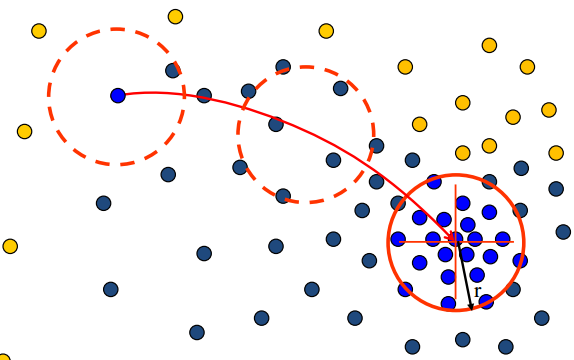
\includegraphics[scale=0.5]{basin1.png}\\
    \textbf{Figure 1:} Adding points within radius $r$ of shift end point\\
\end{center}
			\item Assign all points within radius $c$ of the path of the shift to the same cluster. Imagine initializing a window at one of the points near the path of the shift. Because all windows are shifted in the direction of the most dense area, it is likely that this window will be shifted in the same direction and the point will eventually be assigned to the same cluster. It is common to select the radius $c$ such that $c\le r$.
\begin{center}
	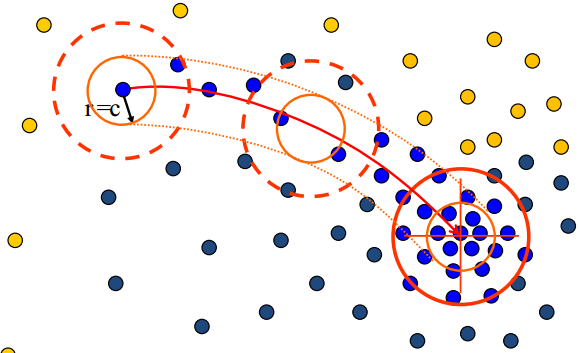
\includegraphics[scale=0.5]{basin2.png}\\
    \textbf{Figure 2:} Adding points within radius $c$ of window path\\
\end{center}
        \end{itemize}
    	\item There is a trade off in selecting the values for $r$ and $c$. The smaller the values, the less nearby points are assigned early and the less computations are saved, but the resulting cluster assignments will have less error if mean-shift was calculated without this method. The larger the values, the more nearby points are assigned resulting in faster speed increases, but also the possibility that the final cluster assignments will be less accurate to standard mean-shift.
    \end{itemize}
\end{itemize}

\subsection{Technical Details}

In order to correctly shift the window you must first identify a nearby area with highest density to calculate the shift vector. This can be accomplished using the multivariate kernel density estimate, which is a way to estimate the probability density function of a random variable.

Given $n$ data points $\mathbf{x}\in\mathbb{R}^d$, the multivariate kernel density estimate, using a radially symmetric (Comaniciu \& Meer, 2002) kernel $K(x)$, is given by
\begin{equation}
\hat{f}_K=\frac{1}{nh^d}\sum_{i=1}^nK\left(\frac{\mathbf{x}-\mathbf{x}_i}{h}\right),
\end{equation}
where $h$ is known as the bandwidth parameter which defines the radius of the kernel. The radially symmetric kernel, $K(x)$ is given by
\begin{equation}
K(x)=c_kk(||x||^2),
\end{equation}
where $c_k$ represents a normalization constant.

Selecting the appropriate $h$ is important for accurately estimating the density. Selecting a value that is too small will result in a small radius and can be subject to noise in the data. Selecting a value that is too large will include too many far away points and result in fewer clusters.

The resulting derivative of the multivariate kernel density estimate is given by
\begin{equation}
\nabla\hat{f}(x)=\frac{2c_{k,d}}{nh^{d+2}}
\left[\sum_{i=1}^ng\left(||\frac{\mathbf{x}-\mathbf{x}_i}{h}||^2\right)\right]
\left[\frac{\sum_{i=1}^n\mathbf{x}_ig\left(||\frac{\mathbf{x}-\mathbf{x}_i}{h}||^2\right)}{\sum_{i=1}^ng\left(||\frac{\mathbf{x}-\mathbf{x}_i}{h}||^2\right)}-\mathbf{x}\right],
\end{equation}
where $g(x) = -K'(x)$ denotes the derivative of the selected kernel profile.

The first term in equation (3), $\frac{2c_{k,d}}{nh^{d+2}}\left[\sum_{i=1}^ng\left(||\frac{\mathbf{x}-\mathbf{x}_i}{h}||^2\right)\right]$, is proportional to the density estimate at $\mathbf{x}$. The second term, $\left[\frac{\sum_{i=1}^n\mathbf{x}_ig\left(||\frac{\mathbf{x}-\mathbf{x}_i}{h}||^2\right)}{\sum_{i=1}^ng\left(||\frac{\mathbf{x}-\mathbf{x}_i}{h}||^2\right)}-\mathbf{x}\right]$, is the mean-shift vector that points towards the direction of maximum density.

\subsection{Mean-Shift Procedure}

From a given point $\mathbf{x}_t$, calculate the following steps in order to reach the center of the cluster.
\begin{enumerate}
	\item Compute the mean-shift vector $\mathbf{m}$ [term 2 from equation (3) above]:
    \begin{equation}
    \mathbf{m}=\left[\frac{\sum_{i=1}^n\mathbf{x}_ig\left(||\frac{\mathbf{x}-\mathbf{x}_i}{h}||^2\right)}{\sum_{i=1}^ng\left(||\frac{\mathbf{x}-\mathbf{x}_i}{h}||^2\right)}-\mathbf{x}\right]
    \end{equation}
    \item Translate the density window using the mean-shift vector:
    \begin{equation}
    \mathbf{x}_i^{t+1}=\mathbf{x}_i^t+\mathbf{m}(\mathbf{x}_i^t)
    \end{equation}
    \item Repeat steps 1 and 2 until convergence
    \begin{equation}
    \nabla f(\mathbf{x}_i)=0
    \end{equation}
\end{enumerate}

\subsection{Kernel Functions}

A kernel function, $K(x)$ is a non-negative function that integrates to 1 over all values of $x$. These requirements ensure that kernel density estimation will result in a probability density function.

Examples of popular kernel functions include:
\begin{itemize}
	\item Uniform (rectangular)
		\begin{itemize}
		\item $K(x)=\frac{1}{2}$ where $|x|\le1$ and 0 otherwise
		\end{itemize}
	\item Gaussian
		\begin{itemize}
		\item $K(x)=\frac{1}{\sqrt[]{2\pi}}e^{-\frac{1}{2}u^2}$
		\end{itemize}
	\item Epanechnikov (parabolic)
		\begin{itemize}
		\item $K(x)=\frac{3}{4}(1-x^2)$ where $|x|\le1$ and 0 otherwise
		\end{itemize}
\end{itemize}

\subsection{Mean-Shift Conclusions}

The mean-shift algorithm has many pros and cons to consider.

Positives of mean-shift:
\begin{itemize}
\item Very general and application independent. 
\item Model-free. Mean-shift does not assume any prior shape of data clusters.
\item Only depends on a single parameter defining the window size. Additional parameters will be required (r and c) if basin of attraction is applied.
\item Finds a variable number of modes. The modes of a distribution function are the local maximums and the locations of these maximums are where the clusters will be centered.
\item Robust to outliers in the data. Mean-shift won't try to force outliers to an existing cluster if they are further than the window size away from all other points.
\end{itemize}

Negatives of mean-shift:
\begin{itemize}
\item Output depends on window size and determining the appropriate window size is not trivial.
\item Computationally relatively expensive to compute the mean-shift from all data points.
\item Does not scale well with dimension of feature space.
\end{itemize}

\section{Object recognition}

\subsection{Object recognition tasks}
The field of object recognition can be broken down into a number of different visual recognition tasks. 

\paragraph{Classification} 
Classification involves teaching computers to properly to label images based on their category of object. It focuses on answering the questions, "is this image of a particular object?" and "does this image contain a particular object?" Typically, classification questions have yes or no answers. For example, typical classification questions could ask if the image contains a building or if the image is of a lake.

\paragraph{Image search} 
This recognition task involves searching a collection of photos for photos of a particular object, like on Google Photos.

\paragraph{Organizing photo collections} 
Object recognition can help organize photo collections based upon location of the photos, similarity of activities, the people who appear in the photos, and other recognizable objects.

\paragraph{Detection}
Detection focuses on the question, "where is a particular object in the image?" Traditional detection methods search for a bounding box that contains the object in question. Using segmentation techniques, the object can also be more specifically selected from the pixels in the image, for what is called accurate localization. \\
Detection can also be targeted at finding geometric and semantic attributes. For example, detection tasks include asking questions such as "is the traffic light red?", "what angle do two buildings make with one another?". Other common attributes found by detection include the distance objects are from one another, and what view of the object the image has.

\paragraph{Single Instance Recognition}
Instead of searching to generally categorize objects, single instance recognition seeks to recognize a particular object or landmark in images. For example, we may want to determine if the picture contains the Golden Gate Bridge or just a bridge. Or, we may want to find a box of a specific brand of cereal.

\paragraph{Activity or event recognition} Activity or event recognition is used to detect what is occurring in a photo. For example, we can ask what people are doing or if the event is a wedding.

\subsection{Challenges}
The challenges to building good object recognition methods include both image and category complications. Since computers can only see the pixel values of images, object recognition methods must account for a lot of variance.

\paragraph{Category numbers}
Studies have shown that humans can recognize roughly 10,000 to 30,000 categories of objects. Currently, the best visual recognition methods can work with about 200 categories for detection, and 1,000 for classification. There are many researchers working to build image datasets to improve object recognition, and recognition with more categories is the subject of many competitions!

\paragraph{Viewpoint variation} There are many potential ways to view an object, and the change in viewpoint can lead an object to look very different.

\paragraph{Illumination} Different levels of light, particularly low light or a different light direction, will cause shadows to shift and the details of an object to become obscured.

\paragraph{Scale} Objects belonging to one category can come in a variety of sizes. If a classification is only trained on a particular size of object, then it will fail to recognize the same object in a different size. One way to solve this bias would be to figure out a way to make better datasets that account for scale variation.

\paragraph{Deformation} Objects can change form and look very different, while still being considered the same object. For example, a person can be photographed in a number of poses, but is still considered a person if they're bending over or if their arms are crossed.

\paragraph{Occlusion} Objects may be occluded, which could hide aspects of their characteristic geometry. While occlusion may be an excellent tool for artists (see Magritte), it is a challenge for computers.

\paragraph{Background clutter} Similarities between the texture, color, and shapes in the background and the foreground can make it difficult to detect an object by blending in the object and/or causing it to appear differently.

\paragraph{Intra-class variation} Within one class of objects, there can be a lot of variation in shape. For example, everything from a barstool to a lounge chair, and a beanbag to an abstract artistic bench can be considered a chair. 

\section{K-nearest neighbors}

\subsection{Supervised learning}
We can use machine learning to learn how to label an image based upon its features. The goal of supervised learning is to use an existing data set to find the following equation:
\begin{equation}
y=f(\mathbf{x})
\end{equation}
In the above equation, $y$ is the output, $f$ is the prediction function, and $\mathbf{x}$ is a set of features from an image.\\

There are two phases of supervised learning: the train and the test phase. In the train phase, we fit an equation, $f$, to the training data set $\{(x_1, y_1) ... \}$, which matches sets of image features to known identifier labels. $f$ can be estimated by minimizing the prediction error, the difference between $y$ and $f(\mathbf{x})$. \\

In the second phase, the test phase, we evaluate our equation, $y=f(x)$, using a new test example that has never been seen by $f$ before. We can compare $f(\mathbf{x})$, and its expected output, $y$, to evaluate if the prediction function works on a new image. If the prediction function does not work on new images, it's not very useful!\\

One way to use supervised machine learning is to learn the decision rules for a classification task.  A decision rule divides input space into decision regions that are separated by decision boundaries.

\begin{center}
	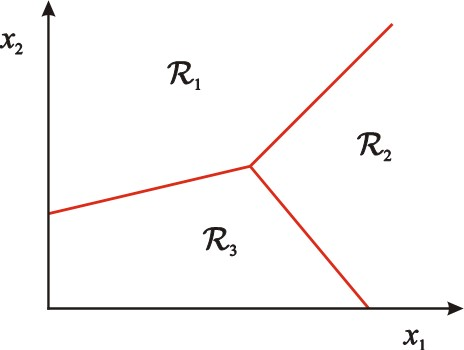
\includegraphics[scale=0.5]{decision_boudnaries.jpg}\\
    \textbf{Figure 3:} Decision regions and decision boundaries (in red) for three categories, $R_1$, $R_2$, and $R_3$ over a feature space with two dimension. \citeauthor{lecture11}\\
\end{center}

\subsection{Nearest neighbor classifier}
The nearest neighbor classifier is an algorithm for assigning categories to objects based upon their nearest neighbor. We assign a new test data point the same label as its nearest training data point.\\

Nearest neighbors are found using the Euclidean distance between features. For a set of training data, where $X^n$ and $X^m$ are the n-th and the m-th data points, the distance equation is written as:
\begin{equation}
Dist(X^n, X^m) = ||X^n - X^m||^2 = \sqrt{\sum_{i}(X^n_i - X^m_i)^2}
\end{equation}

The definition of the nearest neighbors classifier allows for complex decision boundaries that are shaped around each data point in the training set. \\

\subsection{K-nearest neighbors classifier}
We can enhance the nearest neighbors classifier by looking at the k nearest neighbors as opposed to just the nearest neighbor. The k-nearest neighbor classifier calculates the k nearest neighbors, and labels a new object by a score calculated over this set of nearest neighbors. A commonly used metric is to assign a new object to the category that a majority of their nearest neighbors belong to. Heuristics are used to break ties, and are evaluated based upon what works the best. \\

\begin{center}
	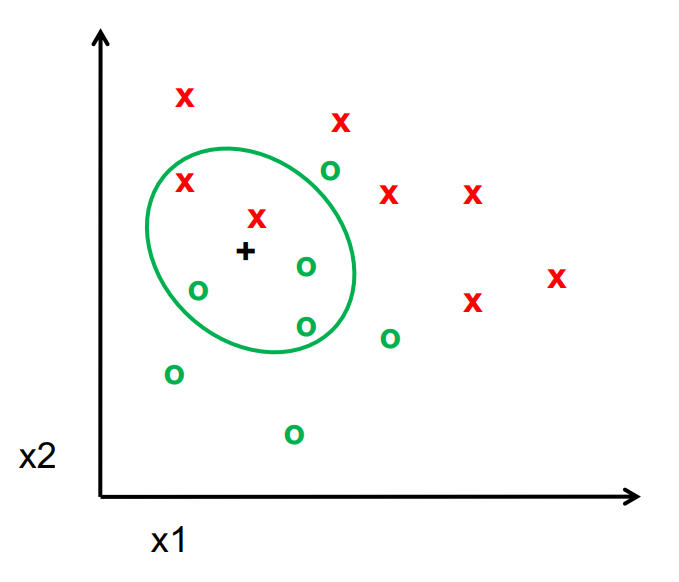
\includegraphics[scale=0.35]{knearestneighbors.png}\\
    \textbf{Figure 4:} For the \textbf{+} data point, the green circle represents it's k-nearest neighbors, for $k=5$. Since three out of five of its nearest neighbors are green circles, our test data point will be classified as a green circle. \cite{lecture11} \\
\end{center}

Like the nearest neighbor classifier, the k-nearest neighbor algorithm allows for complex decision boundaries using a relatively simple equation!

\subsection{Pros of using k-nearest neighbors}

\begin{itemize}
    \item K-NN is a very simple algorithm-- a good one to try out at first
    \item K-NN has very flexible decision boundaries.
    \item (Out of scope for this class) With infinite examples, 1-NN provably has error that is at most twice Bayes optimal error.
\end{itemize}

\subsection{Problems with k-nearest neighbors}


\subsubsection{Choosing the value of k}

It's important to choose the proper value of K when using the K-nearest neighbor algorithm. If the value of K is too small, then the algorithm will be too sensitive to noise points. If the value of K is too high, then the neighborhood may include points from other classes. Similarly, as K increases, the decision boundaries will become more smooth, and for a smaller value of K, there will be more smaller regions to consider.

\begin{center}
	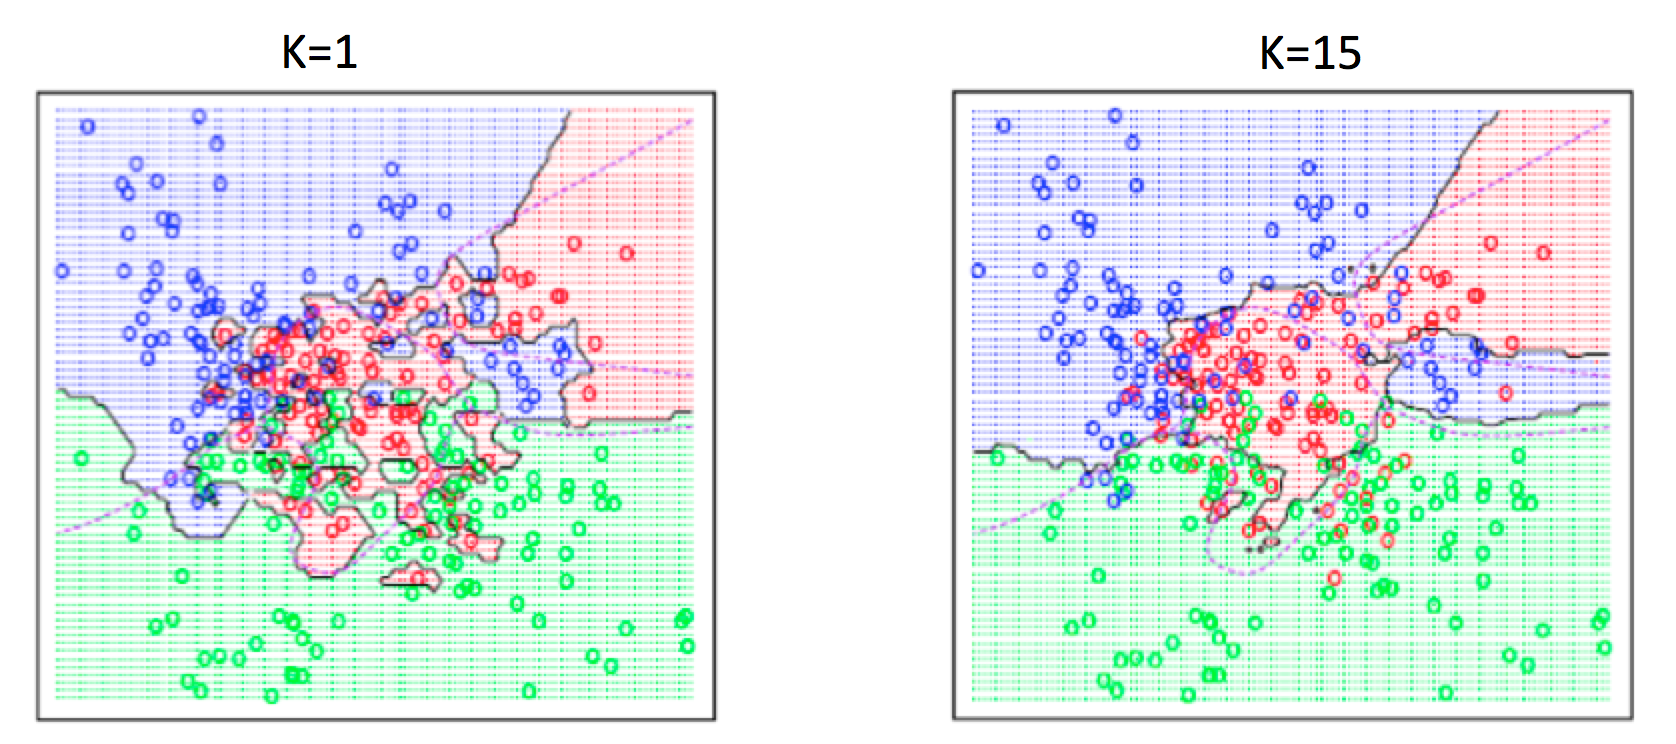
\includegraphics[scale=0.5]{ChoosingValueOfK.png}\\
    \textbf{Figure 1:} Comparing the result of choosing K=1 vs. K=15\\
\end{center}

\textbf{Solution}: Cross validate!\newline
One way to find the proper value of K is to create a holdout cross validation/development set from the training set. From there, we would adjust the hyper parameters (e.g, K) on the development set to maximize training, and then 'test' the development set's accuracy. We would then change the validation set from the training set and repeat until we find the best value of K.

\subsubsection{Euclidean measurement}

Another issue that can arise with the K-nearest neighbor algorithm is that using the Euclidean measure might provide counter-intuitive results. See example below:

\begin{center}
	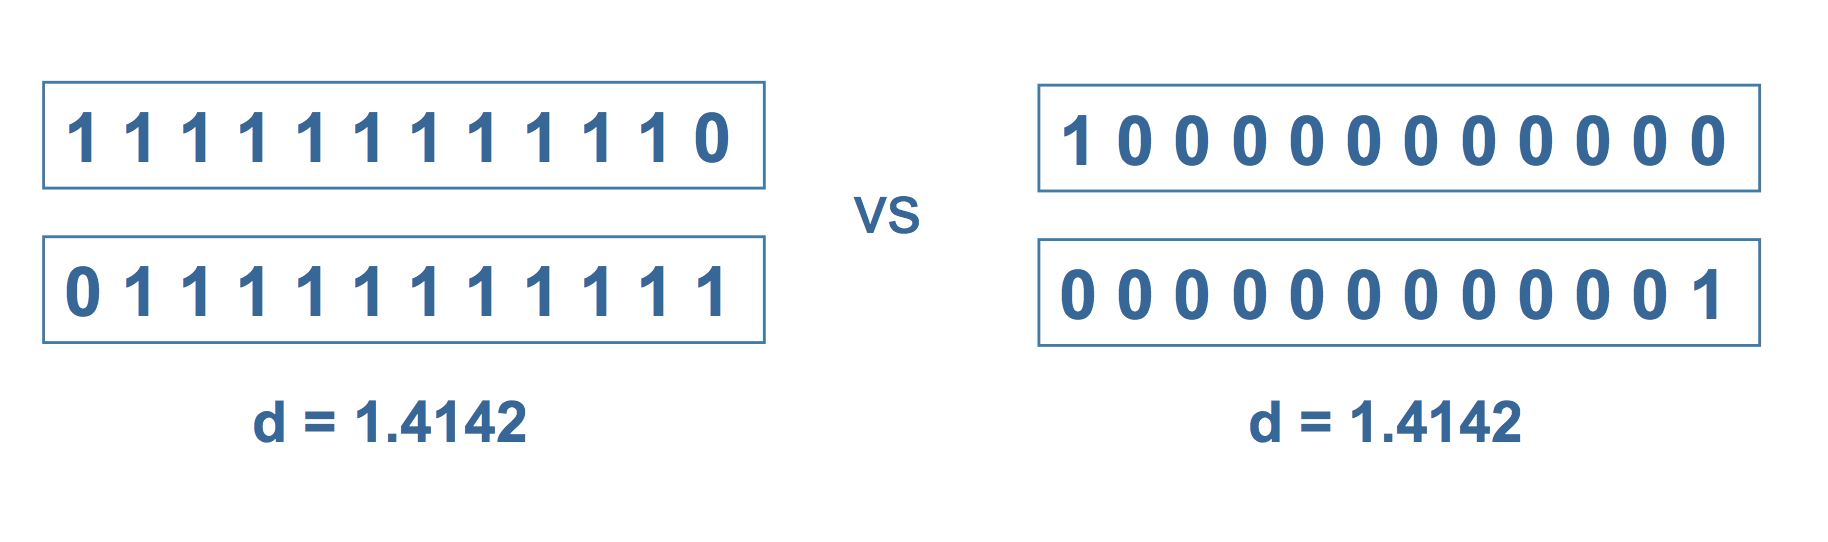
\includegraphics[scale=0.35]{EuclideanIssue.png}\\
    \textbf{Figure 3:} Different values, but using the Euclidean measure equates them to be the same\\
\end{center}

\textbf{Solution}: Normalize!\newline
Normalizing the vectors to unit length will guarantee that the proper Euclidean measurement is used.


\subsubsection{Curse of dimensionality}

When using the K-nearest neighbor algorithm, one issue we need to keep in mind is how to deal with larger dimensions. When the dimensions grow, we need to cover a larger space to find the nearest neighbor. This makes it take longer and longer to calculate the nearest points, and the algorithm will run slower. This also means we will need to have a greater number of examples to train on. Currently, there is no best solution to the dimensionality problem. \newline

\begin{center}
	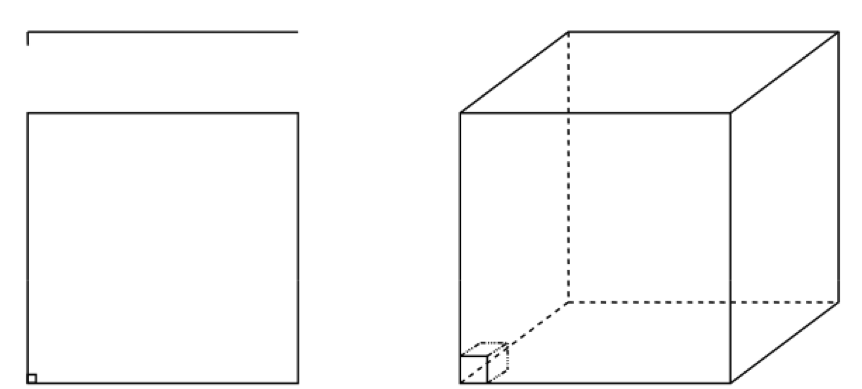
\includegraphics[scale=0.35]{DimensionalityIssue.png}\\
    \textbf{Figure 4:} Larger dimensions require long calculation times\\
\end{center}

\textbf{Problem}: Assume there are 5000 points uniformly distributed in the unit hypercube, and we want to apply 5-NN (Nearest Neighbor). Suppose our query point is at the origin:
\begin{itemize}
    \item In 1 dimension, we must go a distance of $\frac{5}{5000}$=0.001 on the average to capture 5 nearest neighbors
    \item In 2 dimensions, we must go $\sqrt{0.001}$ to get a square that contains 0.001 of the volume
    \item In $d$ dimensions, we must go $(0.001)^{\frac{1}{d}}$
\end{itemize}



\textbf{Note}: K-nearest neighbors is just one of the many classifiers to choose from. That being said, it's not always easy to choose the "best" model for your data. It's best to think about how well you can generalize your model (i.e., how well does your model generalize from the data it was trained on to a new set?). 




\subsection{Bias-variance trade-off}: 

The key to generalization error is to get low, generalized error, by finding the right number/type of parameters. There are two main components of generalization error: bias and variance. Bias is defined as how much the average model over all the training sets differs from the true model. Variance is defined as how much the models estimated from different training sets differ from each other. We need to find the right balance between bias and variance, hence, the bias-variance trade-off. Models with too few parameters are inaccurate because of a large bias (not enough flexibility). Similarly, models with too many parameters are inaccurate because of a large variance (too much sensitivity to the sample). To types of incorrect fitting will be listed below:
\\~\\
\textbf{Underfitting}: The model is too "simple" to represent all of the relevant class characteristics.
\begin{itemize}
    \item High bias and low variance
    \item High training error and high test error
\end{itemize}
\textbf{Overfitting}: The model is too "complex" and fits irrelevant characteristics (noise) in the data.
\begin{itemize}
    \item Low bias and high variance
    \item High training error and and high test error
\end{itemize}

\begin{center}
	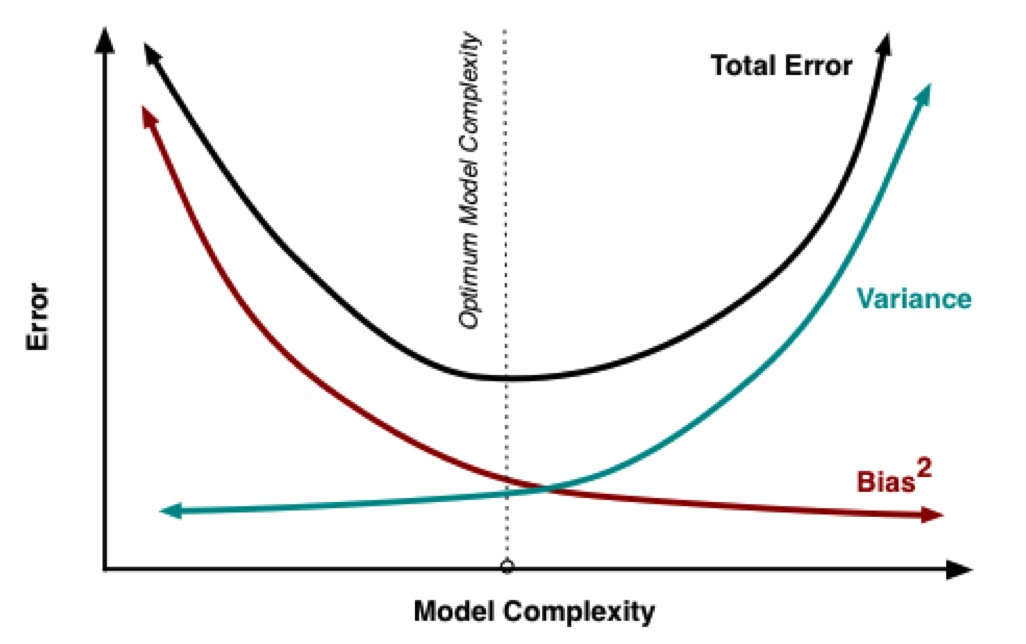
\includegraphics[scale=0.35]{Bias-VarianceTrade-Off.png}\\
    \textbf{Figure 5:} A graph that depicts the trade-off between bias and variance.\\
\end{center}
\end{document}


% References
\small
\bibliographystyle{plain}
\bibliography{bibliography}
\end{document}
